%
% Einleitung zum Skript über lineare Algebra
%
% (c) 2012 Prof Dr Andreas Mueller, Hochschule Rapperswil
%
\chapter*{Einleitung}

Die lineare Algebra stellt sich als Grundlage einer grossen
Zahl von Theorien heraus.
Aufgabe dieser Vorlesung ist, die
Grundlagen dieser Theorie sowie die wichtigsten Anwendungsthemen
zu vermitteln.
Um die Darstellung der Theorie nicht zu stark zu unterbrechen,
werden grösser Anwendungen in separaten Abschnitten am Ende
jedes Kapitels beschrieben.

\section*{Behandelte Themen}
\subsection*{Kapitel 1: Lineare Gleichungssysteme}
Die Lineare Algebra beschäftigt sich zunächst mit der Lösung linearer
Gleichungen.
Dazu werden im ersten Kapitel einige Methoden bereitgestellt,
und es wird diskutiert, unter welchen Voraussetzungen ein
Gleichungssystem keine, genau eine oder unendlich viele
Lösungen hat.
Die Techniken motivieren auch einen neuen Kalkül, die Matrizenrechnung,
welcher das Rechnen mit Zahlen und Vektoren, das vielen
Studierenden bereits bekannt ist, auf beliebige Dimensionen erweitert,
und zudem ein Produkt einführt.

Es geht nicht darum, mit ein paar zusätzlichen Variablen umgehen
zu können.
Moderne Strömungsmodelle beschreiben die Strömung durch die
Geschwindigkeitsvektoren an jedem Punkt eines Millionen von Punkte
umfassenden räumlichen Gitters.
Gesucht werden also Lösungsverfahren, die mit $n>10^6$ Unbekannten
umgehen können.

\subsection*{Kapitel 2: Determinanten}
Für Gleichungssysteme mit gleich vielen Gleichungen wie Unbekannten
kann man ein Art Kennzahl finden, welche direkt Aussagen kann,
ob ein Gleichungssystem eine eindeutige Lösung hat.
Erstaunlicherweise ist die so definierte Grösse, die Determinante,
noch viel universeller.
Man kann damit auch direkt ein Gleichungssystem lösen, oder
die inverse Matrix berechnen.
Ausserdem lässt sich die Determinante zur Flächen- und Volumenberechnung
verwenden, und man kann damit das Vektorprodukt definieren.

\subsection*{Kapitel 3: Affine Vektorgeometrie}
Die abstrakte Sprache der Vektoren und Matrizen kann auf die Geometrie
angewendet werden.
Linear unabhängige Vektoren und Linearkombinationen führen auf den
Begriff der Basis und der Koordinatensysteme.
Geraden und Ebenen können einerseits als Teilmengen des Raumes
betrachtet werden, aber auch als Lösungsmenge eines Gleichungssystems.
Probleme der Lage können darin formuliert und auf die Lösung von
linearen Gleichungssystemen zurückgeführt werden.

\subsection*{Kapitel 4: Skalarprodukt}
Die affine Vektorgeometrie kennt weder den Begriff der Länge noch den
des Winkels.
Im Kapitel~3 konstruierte Abbildungen haben rechte Winkel und gleich
lange Strecken zerstört.
Wenn man Längen und Winkel berücksichtigen will, braucht man ein
algebraisches Werkzeug, mit dem sich Längen diese berechnen lassen.
Es zeigt sich, dass Basen mit senkrecht stehenden Vektoren besonders
elegante Eigenschaften haben.

\subsection*{Kapitel 5: Orientierung und Vektorprodukt}
Die Determinante gibt einer Basis eines Vektorraumes eine zusätzliche
Struktur.
In der Ebene erlaubt sie, Uhrzeigersinn und Gegenurzeigersinn zu 
unterscheiden.
Im dreidimensionalen Raum erklärt sie den Unterschied zwischen
rechter und linker Hand.
In drei Dimensionen führt Sie ausserdem auf das Vektorprodukt, welches
viele interessante Anwendungen in der Geometrie und Physik.

\subsection*{Kapitel 6: Eigenschaften linearer Abbildungen}
In den Kapiteln~3--6 ist immer wieder der Begriff der linearen
Abbildung aufgetaucht.
In Kapitel 6 wird systematisch untersucht, wie sich mit dem Skalarprodukt
und der Orientierung Eigenschaften von linearen Abbildungen formulieren
lassen
und so etwas Ordnung in die Menge der linearen Transformationen
gebracht werden kann.

In der Praxis werden damit Transformationen des Raumes beschrieben
z.~B.~für Computergraphik (Games) oder die Robotik.
Auch Computer-Vision verwendet sie zur Analyse von Kamerabildern
(siehe auch den Abaschnitt Kamerageometrie weiter unten).
3D-Graphikkarten implementieren diese Operationen in der Hardware.


\subsection*{Kapitel 7: Matrixzerlegungen}
Der Gauss-Algorithmus aus Kapitel~1 kann auch als eine
Zerlegung einer Matrix in zwei Dreiecksmatrizen formuliert werden.
Es lassen sich aber auch andere Zerlegungen finden, die je
nach Anwendungsfall geeigneter sind.

\subsection*{Kapitel 8: Eigenwerte und Eigenvektoren}
Das wahrscheinlich wichtigste Problem der lineare Algebra
ist das Eigenwertproblem.
Dieses Kapitel beschreibt das Problem und die Lösung mit Hilfe
des charakteristischen Polynoms.
In einem eigenen Abschnitt werden ausserdem numerische Algorithmen
beschrieben, die Eigenwerte und Eigenvektoren auch für grössere
Matrizen finden können, für welche das charakteristische 
Polynom keinen praktikablen Lösungsweg darstellt.

\section*{Anwendungen}
Jedes Kapitel enthält am Ende auch einen Abschnitt mit grösseren
Anwendungen der Theorie des Kapitels.

\subsection*{Die Kirchhoffschen Gesetze}
Die Kirchhoffschen Gesetze erlauben die Ströme in einem Netzwerk
zu berechnen.
Dieses Problem wurde ursprünglich von Gustav Robert Kirchhoff
formuliert und gelöst.
Als Nebenresultate seiner Theorie
entstand auch eine ganze Menge von Resultaten über Netzwerke.
Zum Beispiel zeigt sich, wie man mit Hilfe von Determinanten
die Zahl der möglichen Spannbäume eines Graphen zählen kann.

\subsection*{Kurvenanpassung}
Die Methode der kleinsten Quadrate liefert auch eine Methode,
mit der man zu einer Menge von Messwerten eine bestmöglich passende
Funktion finden kann.

\subsection*{Wavelets}
Die Orthogonalisierungsmethode erlaubt eine Menge von
Basisfunktionen zu finden, nach denen man eine gesamplete Funktion
besonders effizient entwickeln kann.
Sie bildet die Grundlage für Wavelets, die in der modernen Signalverarbeitung
eine bedeutende Rolle spielen.

\subsection*{Kamerageometrie}
Nicht zuletzt dank der Verbreitung von Kameras in Mobiltelefonen hat
sich die Kamera als optischer Universalsensor etabliert.
Die Verarbeitung der Information in einem Bild ist zwar aufwendig,
aber auch Rechenleistung steht heute fast immer in ausreichendem Masse 
zur Verfügung.
Die Umrechnung zwischen dem dreidimensionalen Raum und dem zweidimensionalen
Bild führt auf eine interessante Anwendung der linearen Algebra.

\subsection*{Google Pagerank}
Suchmaschinen im Internet müssen aus einer potentiell sehr grossen Zahl
von Suchresultaten die treffendsten als erste liefern.
Die einzige Quelle zur Bewertung der Resultate kann nur
das Internet selbst sein.

\section*{Die Karte der linearen Algebra}
Die Karte der linearen Algebra auf der folgenden Seite zeigt ein
paar Begriffe, die in den nachfolgenden Kapiteln erklärt werden.
Der Leser wird aufgefordert, bei Gelegenheit zu dieser Karte
zurückzukommen und zu versuchen, ob er den dargestellten
Zusammenhängen einen Sinn geben kann.

\begin{landscape}
\begin{center}
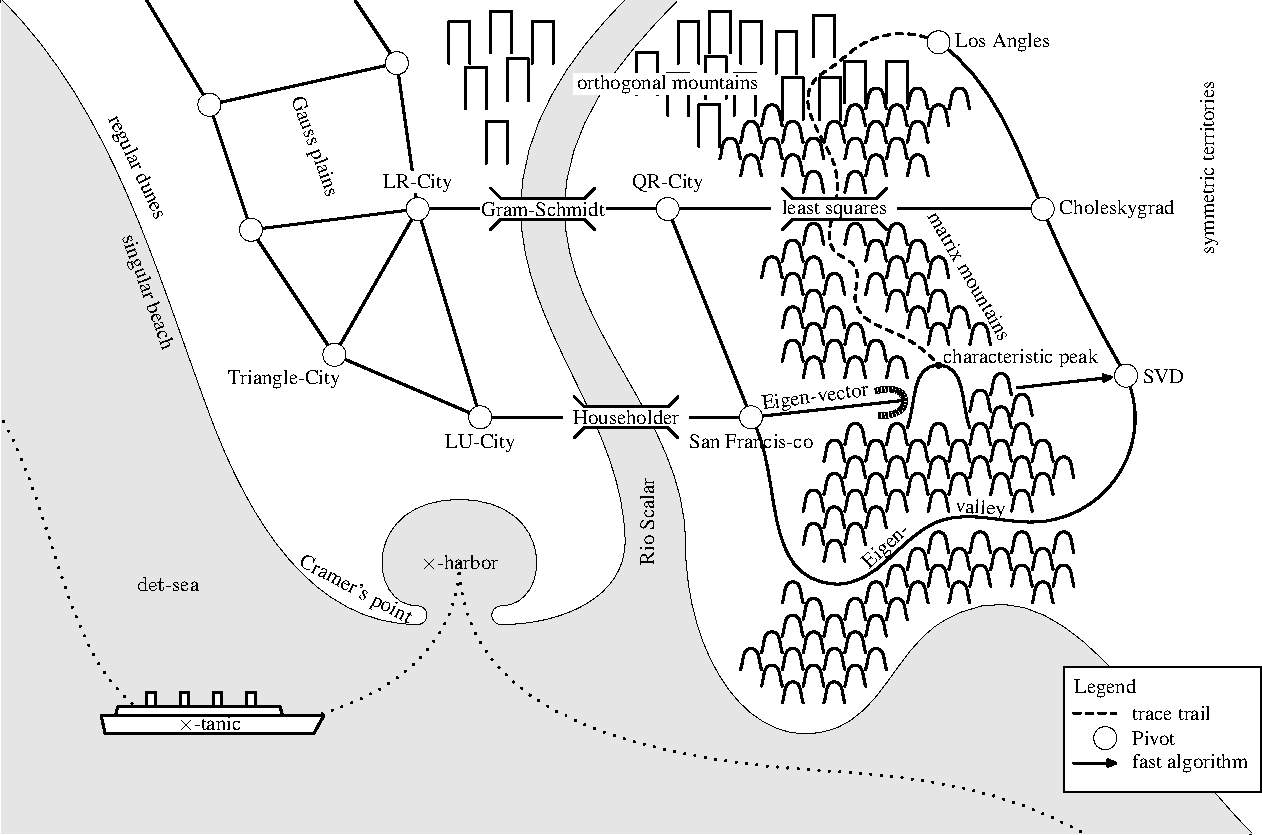
\includegraphics[width=0.95\hsize]{images/linalgmap-1}
\end{center}
\end{landscape}
